% This must be in the first 5 lines to tell arXiv to use pdfLaTeX, which is strongly recommended.
\pdfoutput=1
% In particular, the hyperref package requires pdfLaTeX in order to break URLs across lines.

\documentclass[11pt]{article}

% Remove the "review" option to generate the final version.
\usepackage[]{acl}

% Standard package includes
\usepackage{times}
\usepackage{latexsym}

% For proper rendering and hyphenation of words containing Latin characters (including in bib files)
\usepackage[T1]{fontenc}
% For Vietnamese characters
% \usepackage[T5]{fontenc}
% See https://www.latex-project.org/help/documentation/encguide.pdf for other character sets

% This assumes your files are encoded as UTF8
\usepackage[utf8]{inputenc}

% This is not strictly necessary, and may be commented out,
% but it will improve the layout of the manuscript,
% and will typically save some space.
\usepackage{microtype}
\usepackage{blindtext}


%Including images in your LaTeX document requires adding
%additional package(s)
\usepackage{graphicx}
\usepackage{xcolor}

% If the title and author information does not fit in the area allocated, uncomment the following
%
%\setlength\titlebox{<dim>}
%
% and set <dim> to something 5cm or larger.

\title{Project report: Investigating teaching rule based inference to LLMs}

\author{Julian Fesel \\
\texttt{julian.fesel@icloud.com}
}

\begin{document}

    \maketitle


    \section{Introduction}
    The motivation for this project comes from my current occupation in the railway sector.
    There, routing conflicts between different scheduled trains must be solved by special operatives.
    Most of these decisions follow guidelines that define which trains must be prioritized under which circumstances.

    These guidelines can be quite extensive and intricate and the decisions must be made quickly.
    It is therefore of interest, to try to use LLMs to support the operatives in this task, by providing decision
    recommendations based on the guidelines and a description of the current situation.

    Since the data that would be necessary to work on this topic is currently not available, this project aims to
    investigate a topic that is relevant to this future effort.
    The idea is inspired by approaches I already used in assignment three.
    There I tried to improve the performance of few-shot prompting by enhancing the prompt with a step-by-step guide
    how to arrive at a solution and enriching the provided few-shot examples with a chain-of-though like reasoning based
    on the guide.
    The CoT reasoning was created by GPT-4.

    It was very interesting for me to see, that in context learning approaches performed much worse than the ones based
    on fine-tuning.
    This leads me to the question, whether enriching a dataset by a guide and CoT style logic helps during fine-tuning,
    which is now the topic of this project.


    \section{Hypotheses}\label{S:hypothesis}

    The core hypotheses of this project can be stated as follows:
    Given a dataset $D = \{D_i\}_{i=1}^N$ of pairs $D_i = (X_i, Y_i)$ , a pre-trained base-model $M$ and
    a larger trainer model $\mathcal{M}$ that is superior to $M$.
    Then the hypothesis of this project is, that the sample-efficiency of fine-tuning $M$ on $D$ can be improved by
    training on a dataset $D^\prime$ derived from $D$.
    The dataset $D^\prime$ is constructed in three steps:
    \begin{enumerate}
        \item Generate a step-by-step guide $\mathcal{G}$ how to derive a particular $Y_i$ from $X_i$ using the trainer model
        $\mathcal{M}$ and a small subsample of the original dataset.
        \item Using the guide and the trainer model, derive the new dataset by inserting the guide $\mathcal{G}$ in the
        original prompts $X_i$ and enhance the corresponding $Y_i$ by CoT-style logic generated by the trainer model $\mathcal{M}$.
        \item Filter the new dataset for pairs $D^\prime_i = (X^\prime_i, Y^\prime_i)$ where the CoT in $Y^\prime_i$
        leads to the correct answer $Y^\prime_i$.
    \end{enumerate}

%    \begin{itemize}
%        \item Given a dataset $D = \{D_i\}_{i=1}^N$ of prompt/answer pairs $D_i = (X_i, Y_i)$ and a pre-trained
%        base-model $M$.
%        The sample-efficiency
%        \begin{itemize}
%            \item zero or few shot baseline (no rules)
%            \item teacher model or self extract guide from examples + gen new samples with problem+guide+answer
%            \item iterative improvement of ruleset
%            \item full/lora/qlora fine-tuning baseline
%            \item full/lora/qlora fine-tuning on guide dataset
%            \item actor/critic approaches on top of reasoning
%            \item full/lora/qlora fine-tuning on other datasets with rules. check influence
%            \item compare how findings relate to http://arxiv.org/abs/2310.09158
%        \end{itemize}
%        \item
%    \end{itemize}


    \section{Data}

    The hypothesis is tested on the ReCOGS (\textbf{CO}mpositional \textbf{G}eneralization Challenge based on
    \textbf{S}emantic Interpretation) dataset \cite{wu_recogs_2024, kim_cogs_2020}.
    This choice is made due to the fact that I am already familiar with it from the previous assignment, and that the
    dataset constitutes a good compromise between size, complexity and relatedness to real-world applications.
    It is also well suited for the step-by-step guide generation that is part of this projects' hypothesis.

    A slight modification of the original ReCOGS dataset is performed, by renumbering the semantic components of the
    logical form of the sentence to always be monotonically increasing from one.
    An example of a resulting pair of sentence and logical is shown in figure \ref{fig:recogs_base}.

    \begin{figure}
        \small
        \begin{description}
            \item[\texttt{Sentence $X_i$:}] \texttt{A scientist gave the radio to Emma .}
            \item[\texttt{Logical Form $Y_i$:}] \texttt{scientist ( 1 ) ; * radio ( 2 ) ; Emma ( 3 ) ; give ( 4 ) AND agent ( 4 , 1 ) AND theme ( 4 , 2 ) AND recipient ( 4 , 3 )}
        \end{description}
        \caption{Example of a ReCOGS data pair after applying the renumbering.}
        \label{fig:recogs_base}
    \end{figure}


    \section{Metrics}

    The evaluation of the hypothesis stated in \ref{S:hypothesis} is based primarily on the exact-match metric as used
    in the assignment.
    Using this metric the accuracy on a hold-out testset is calculated for various fine-tuned models.
    This allows to compare the performance of the models during the training at specific epochs and for different sizes
    of training datasets.
    This comparison is then used to conclude on the initial hypothesis.


    \section{Models}

    As the base model $M$ that is fine-tuned, a Mistral-7B model is used \cite{jiang_mistral_2023}.
    Specifically, an instruct tuned and 4-bit quantized version of the model is chosen.
    The reasons behind this choice are the following:
    \begin{itemize}
        \item The model is open-source and has a permissible license
        \item It represents a good tradeoff between performance and size
        \item Using QLoRa \cite{dettmers_qlora_2023}, the model can be fine-tuned on affordable hardware, comparable to a T4-GPU from Nvidia
    \end{itemize}

    For the trainer model $\mathcal{M}$, the newest version of GPT-4 (\texttt{gpt-4-0125-preview}) is used via the
    commercial API-offering of OpenAI \cite{openai_gpt-4_2024}.


    \section{General Reasoning}\label{S:reasoning}

    The project can be segmented into the following steps:

    \begin{enumerate}
        \item Sample a small subset $D_\mathrm{sub}$ of 20 datapoints from the training segment of the renumbered ReCOGS dataset.
        \item Using a handcrafted prompt and GPT-4, generate a step-by-step guide $\mathcal{G}$ from $D_\mathrm{sub}$.
        \item Sample another subset $D_\mathrm{train}$ of 200 datapoints from the training segment of the renumbered ReCOGS dataset.
        \item Use a handcrafted prompt together with the guide $\mathcal{G}$ to enrich $D_\mathrm{train}$
        with CoT-style reasoning using GPT-4. This leads to a new training dataset $D_\mathrm{train}^\prime$.
        \item Fine-tune two different Mistral model on $D_\mathrm{train}$ and $D_\mathrm{train}^\prime$ for 10 epochs.
        The models are fine-tuned once with the full datasets and then also with subsets of 10, 50 and 100 samples.
        \item Evaluate each model on the same sample of 200 datapoints from the gen segment of the ReCOGS dataset.
        \item Visualize the accuracy of the different models at various stages during the fine-tuning.
    \end{enumerate}


    \section{Summary of Progress}

    I have finished going through the steps outlined in section \ref{S:reasoning}. The first visualizations of the results
    can be seen in figures \ref{fig:acc_vs_epoch} and \ref{fig:acc_vs_data}.

    Unfortunately the results so far do not provide strong support for the hypothesis stated in section \ref{S:hypothesis}.
    Even though the models trained on $D^\prime$ show better performance on very small fine-tuning datasets and in early
    epochs, this advantage vanishes for larger --- but still small --- training datasets.

    However, the results are interesting and informative, and allow for a thorough discussion and analysis.
    So far, there are no critical blockers in sight and the most important parts including the generation of the derived
    dataset and fine-tuning are already done.

    The next steps of the project will focus on writing the final report and a careful analysis of the results so far.
    They can be summarized as:
    \begin{itemize}
        \item Perform a detailed analysis of the results.
        \item Evaluate the performance of the approach with step-by-step prompt without any fine-tuning
        and add it to the visualizations.
        \item Analyse the performance with respect to the number of tokens used for training.
        \item Compare the costs and fine-tuning durations of the different fine-tuning regimes.
        \item Add a discussion on the pros and cons of the approach discussed in this project. Which applications might
        benefit from this approach?
    \end{itemize}

    \begin{figure}
        \centering
        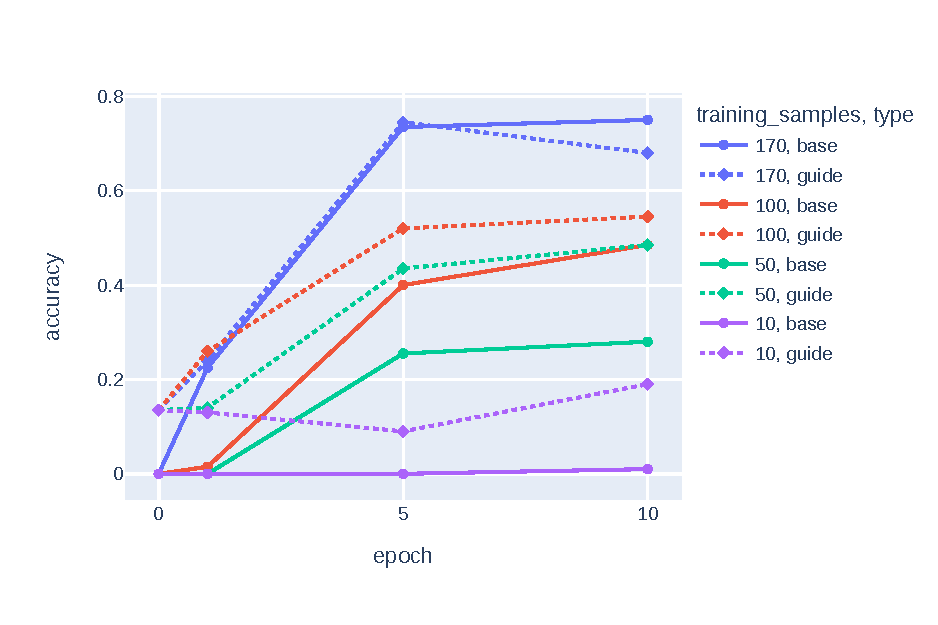
\includegraphics[width=0.45\columnwidth]{../plots/accuracy_vs_epoch.pdf}
        \caption{The accuracy of the Mistral-7B models at different points during the fine-tuning.
        \emph{Base} refers to the standard ReCOGS dataset after renumbering and \emph{guide}
        refers to the CoT-enhanced dataset $D^\prime$.
        }
        \label{fig:acc_vs_epoch}
    \end{figure}

    \begin{figure}
        \centering
        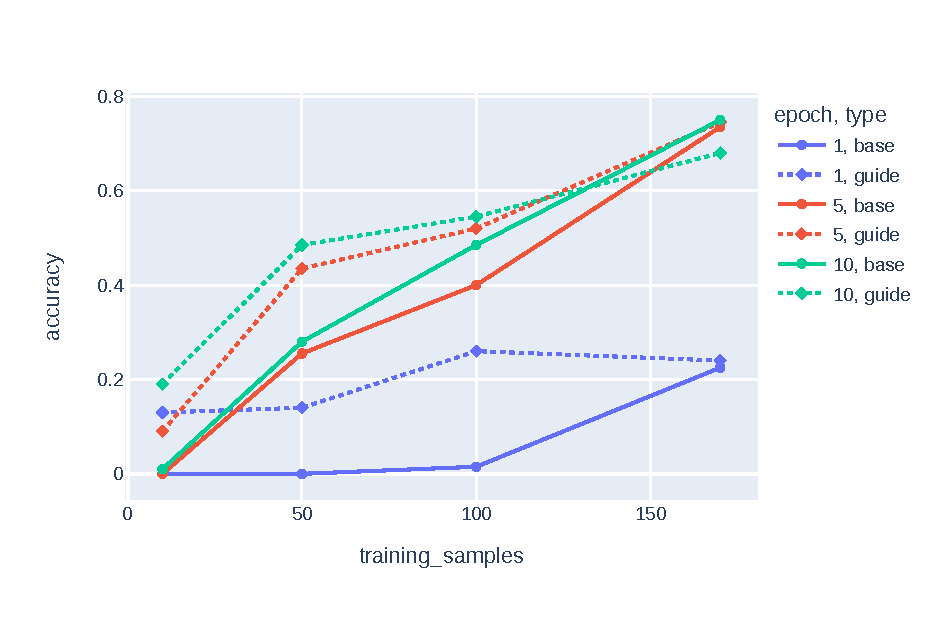
\includegraphics[width=\columnwidth]{../plots/accuracy_vs_data.pdf}
        \caption{The accuracy of the Mistral-7B models with respect to the size of the dataset used for fine-tuning.
        \emph{Base} refers to the standard ReCOGS dataset after renumbering and \emph{guide}
        refers to the CoT-enhanced dataset $D^\prime$.
        }
        \label{fig:acc_vs_data}
    \end{figure}

    % Entries for the entire Anthology, followed by custom entries
    \bibliography{anthology,custom,julian}

    \appendix


    \section{Prompts and guide}\label{sec:appendix}

    \begin{figure*}
        \small
        \texttt{You must come up with a general step by step guide, how to create the logical form from a given sentence.\\
        The guide should also explain the syntax and symbols that the specific logical form requires.\\
        The guide must be compact and use only as many words as are needed to cover all necessary rules. It must not contain any markdown formatting.\\
        The last step of the guide should only return the full correct logical form.\\
        \\
        Using one of the example pairs, give a demonstration how you use the guide to convert a sentence into its correct logical form.\\
        \\
        -----\\
        Examples:\\
        {\color{red}\{Twenty example pairs are inserted here\}}
        }
        \caption{The prompt sent to GPT-4 to generate a step-by-step guide for solutions of the ReCOGS dataset.}
        \label{fig:guide_prompt}
    \end{figure*}

    \begin{figure*}
        \small
        \begin{verbatim}
Syntax and symbols:
- "*" indicates nonspecific or generalized nouns.
- Numerals (1, 2, 3, ...) are used to uniquely identify nouns and verbs.
- Parentheses are used to group the arguments of functions and relations.
- Semicolons are used to separate independent statements or clauses.

Guide:
1. Identify nouns: Assign each noun a unique numeral (start with 1,
increment for each new noun). If a noun is indefinite or nonspecific,
prefix it with *.

2. Identify the main verb: Assign the next numeral in sequence to the main verb.

3. Determine verb dependencies: For each action (verb), identify its agent (doer),
theme (receiver), or recipient if applicable.
    - Use "agent" for the doer of the action.
    - Use "theme" for the direct object or the focus of the action.
    - Use "recipient" for the indirect object or beneficiary of the action.
    - Use "nmod." for prepositional relations, specifying the relation (e.g.,
        "nmod.in", "nmod.on").

4. Special cases: - For sentences with embedded clauses or secondary actions,
    repeat step 3 for the secondary action within its scope.
    - For sentences indicating possession, use the relation "possessor" and
        "possession".

5. Represent the logical form: - Use semicolon (;) to separate statements.
    - Use parentheses for function arguments, starting with the function
        name (e.g., the verb or relation), followed by the numerical
        identifiers of the relevant nouns.
    - Use "AND" to join multiple conditions or relations related to the same verb.

---
Demonstration with example:

Sentence: "Noah sold a donut to a bear."

Step 1: Identify nouns - Noah ( 1 ); donut ( 2 ); bear ( 3 )
Step 2: Identify the main verb - sold ( 4 )
Step 3: Determine verb dependencies
    - Noah is the agent who performs the action of selling, so he's the "agent".
    - The donut is the item being sold, so it's the "theme".
    - The bear is the recipient of the donut, so it's the "recipient".
Step 4: Special cases: - Not relevant
Step 5: Represent the logical form Noah ( 1 ); donut ( 2 ); bear ( 3 );
    sell ( 4 ) AND agent ( 4 , 1) AND theme ( 4 , 2) AND recipient ( 4 , 3 )
        \end{verbatim}
        \caption{The step-by-step guide generated by GPT-4 for the ReCOGS dataset.}
        \label{fig:recogs_guide}
    \end{figure*}

    \begin{figure*}
        \small
        \begin{verbatim}
Step 1: Identify nouns - cat ( 1 ); *strawberry ( 2 ); pedestal ( 3 ); boy ( 4 )
Step 2: Identify the main verb - lended ( 24 )
Step 3: Determine verb dependencies
    - The cat is the agent of lending, so it's the "agent".
    - The strawberry is the item being lent, so it's the "theme".
    - The boy is the recipient of the strawberry, so it's the "recipient".
    - The strawberry is on the pedestal, which is a prepositional relation.
Step 4: Special cases - The relation between the strawberry and the pedestal
    is specified with "nmod.on".
Step 5: Represent the logical form cat ( 1 ); *strawberry ( 2 ); pedestal ( 3 );
    boy ( 4 ); nmod.on ( 2 , 3 ) AND lend ( 24 ) AND agent ( 24 , 1 ) AND
    theme ( 24 , 2 ) AND recipient ( 24 , 4 )
        \end{verbatim}
        \caption{The step-by-step solution generated by GPT-4 for the sentence
        "A cat lended the strawberry on a pedestal to a boy."}
        \label{fig:gpt4_guide}
    \end{figure*}

    \begin{figure*}
        \small
        \texttt{
        You are given a sentence and must convert it to a specific logical form that
        represents the semantics of the sentence. To do this you must follow a step
        by step guide that you are provided with below. You must follow the steps and
        generate answers for each of the steps, while using as few words as possible.
        The answer to each step should lead to the logical form, which you return in
        the last step. For support, you are also given an example of how to use the
        step by step guide to convert a given sentence to its logical form.\\
        \\
        -----\\
        Step by step guide and demonstration:\\
        {\color{red}\{The step-by-step guide generated by GPT-4 is inserted here (see fig. \ref{fig:recogs_guide})\}}\\
        \\
        -----\\
        Sentence to convert:\\
            {\color{red}\{The sentence to convert is inserted here.\}}
        }
        \caption{The prompt used for inference, for the case with CoT-style solution.}
        \label{fig:prompt_using_guide}
    \end{figure*}

\end{document}

